\documentclass[a4paper]{article}

\usepackage{amsmath}
\usepackage{amssymb}
\usepackage{parskip}    % skip line
\usepackage{fullpage}   % margins
\usepackage{hyperref}   % hyper references and document setup
\usepackage{xcolor}     % colors
\usepackage{listings}   % format code
\usepackage{biblatex}   % references
\usepackage{graphicx}   % images

\usepackage{lpi}

% Se scritta in italiano:
%\usepackage[italian]{babel}

\addbibresource{./references.bib}
\graphicspath{ {./media} } % sections/images

\title{%
    Trimap Matting \\
    \phantom{} \\
    \large Scuola d'Arti e Mestieri di Trevano (SAMT) \\
    \large Documentation
}

\author{Paolo Bettelini}

\date{}

\lpisetup%
    {Trimap Matting}

\begin{document}

\maketitle

\pagebreak


\tableofcontents

\pagebreak

\section{Introduction}

\subsection{Abstract}

\subsection{Information}


This is a project of the Scuola Arti e Mestieri di Trevano (SAMT) under the following circumstances

\begin{itemize}
    \item \textbf{Section}: Computer Science
    \item \textbf{Year:} Fourth
    \item \textbf{Class:} Progetti Individuali
    \item \textbf{Supervisor:} Geo Petrini
    \item \textbf{Title:} Trimap Matting
    \item \textbf{Start date}: 2022-09-29
    \item \textbf{Deadline}: 2022-12-07
\end{itemize}

and the following requirements

\begin{itemize}
    \item \textbf{Documentation}: a full documentation of the work done
    \item \textbf{Diary}: constant changelog for each working session
    \item \textbf{Source code}: source code of the project
\end{itemize}

All the source code and documents can be found at
\href{https://github.com/paolobettelini/trimap-matting}
{https://github.com/paolobettelini/trimap-matting}
\cite{gitrepo}.

\pagebreak

\section{Requirements}

\requirement{00}{CLI tool}{1}{1.1}{none}{
    A CLI tool to execute background removal must be developed
}{
    \subreq{00}{0}{The target image must be specified}
    \subreq{00}{1}{The trimap image can be specified}
    \subreq{00}{2}{The soft mask can be specified}
    \subreq{00}{3}{Either the soft mask or the trimap must be specified}
    \subreq{00}{4}{The program can save the generated background mask}
    \subreq{00}{5}{The program can remove the background and replace it with an image}
    \subreq{00}{6}{The program can remove the background and fill it with a color}
    \subreq{00}{7}{The program can remove the background and leave it transparent}
}

\requirement{01}{Image formats}{1}{1.0}{none}{
    Multiple image formats must be supported
}{
    \subreq{00}{0}{The JPG format must be supported}
    \subreq{00}{1}{The PNG format must be supported}
    \subreq{00}{2}{The WebP format must be supported}
}

\requirement{02}{Size check}{1}{1.0}{none}{
    The executable must assert that the target image and trimap are of the same size
}{%
}

\requirement{03}{GUI}{1}{1.0}{none}{
    A GUI application must be developed in other to interact with the program features
}{%
}

\pagebreak

\section{To use}

\begin{lstlisting}[style=Rust, style=boxed]
    let output = log!(
        "Generating soft mask",
        args.verbose,
        matting::generate_mask(&target, &trimap)? // heavy lifting
    );
\end{lstlisting}

\begin{lstlisting}[style=HTML, style=boxed]
    <div>
        <h1>Title</h1>
    </div>
\end{lstlisting}

\begin{lstlisting}[style=JS, style=boxed]
    function ciao() {
        console.log("ee");
    }
\end{lstlisting}

\begin{lstlisting}[style=TOML, style=boxed]
    # asd
    hello = "valore"
\end{lstlisting}

\begin{lstlisting}[style=nginx, style=boxed]
    server {
        server_name = _;
    }
\end{lstlisting}

\pagebreak

\section{CLI}

\subsection{Compilation}

The executable can be compiled using the \texttt{cargo}
package manager.

\begin{lstlisting}[style=boxed]
    $ cd matting-cli
    $ cargo build --release
\end{lstlisting}

This will generate an executable (\texttt{matting-cli})
in \texttt{./target/debug}.
In order to make this executable globally available
we can move it into a folder in the \textsc{\$PATH} enviroment
variable, such as \texttt{/usr/bin}.
We may also modify the executable file name to change its invokation
name.

\begin{lstlisting}[style=boxed]
    $ sudo mv target/release/matting-cli /usr/bin/
\end{lstlisting}

We executable can now be invoked by just writing
\begin{lstlisting}[style=boxed]
    $ matting-cli
\end{lstlisting}

\subsection{Usage}

The followings shows the output of the command upon
setting the \texttt{--help} or \texttt{-h} flag.
\begin{lstlisting}[style=boxed]
Matting CLI

Usage: matting-cli [OPTIONS] --target <TARGET>
                   <--mask <MASK>|--trimap <TRIMAP>>

Options:
  -i, --target <TARGET>        Target image
      --mask <MASK>            Background mask image
      --trimap <TRIMAP>        Trimap image
      --save-mask <SAVE_MASK>  Save mask path
  -o, --output <OUTPUT>        Output image
  -f, --fill <FILL>            Fill background action
  -t, --transparent            Transparent background action
  -r, --replace <REPLACE>      Replace background action
      --verbose                Verbose flag
  -h, --help                   Print help information
  -V, --version                Print version information
\end{lstlisting}

The \texttt{--target} parameter specifies the image
on which the operation needs to be applied.
This parameter is \underline{mandatory}.

The \texttt{--trimap} parameter specifies the trimap
image which will be used to generate the alpha mattes.

The \texttt{--mask} parameter specifies the image
containing the alpha mattes to use.

The parameter \texttt{--trimap} and \texttt{--mask}
are mutually exclusive and one of them is \underline{mandatory}.

The advantage of using \texttt{--mask} over
\texttt{--trimap} is that the alpha mattes are
already given rather than having to be computed.
This can save lots of computational times.
The alpha mattes image can be saved on the file system
by specifying the \texttt{--save-mask} parameter.

There are 3 different operations that can be applied
to the background of the result: \texttt{--transparent},
\texttt{--replace} or \texttt{--fill}.
These operations are mutually exclusive and if one is specified,
the \texttt{--output} parameter must also be set to
specify the path where the resulting image will be saved.
Similarly, if the \texttt{--output} parameter is set
an operation must also be specified.

\textbf{Note:} the argument of \texttt{--color} can be any valid
CSS color. See \cite{csscolors} for the documentation.

The \texttt{--verbose} flag is optional and will print additional
information about what the program is doing and the elapsed
time of each operation.

\subsection{Examples}

The following command generate a mask of the alpha mattes
given a trimap.
\begin{lstlisting}[style=boxed]
    $ matting-cli -i target.jpg --trimap trimap.png
        --save-mask mask.png
\end{lstlisting}

%

The following shows the output of the program when the \texttt{--verbose}
flag is set. This command computes the alpha mattes given a trimap,
then it saves the generated mask, fills the background of the image
with the color red and then saves the result.
\begin{lstlisting}[style=boxed]
    $ matting-cli -i target.jpg --trimap trimap.png
        --save-mask mask.png -o out.png --fill red --verbose
    
    Reading target image... Done! [4.021485ms]
    Reading trimap image... Done! [1.976477ms]
    Generating soft mask... Done! [7.104532642s]
    Reading target image... Done! [178.884124ms]
    Saving soft mask... Done! [509.050896ms]
    Filling background with color... Done! [117.90393ms]
    Saving output... Done! [954.085622ms]
\end{lstlisting}

\pagebreak

\section{Trimap Matting}

Matting is a technique used to extract an object
from an image.
Trimap matting is a term used to refer to the process
of generating alpha mattes\cite{matte} for an object
% https://en.wikipedia.org/wiki/Matte_(filmmaking)
in an image given an initial
approximation of its borders.

The goal of this process is to determine
how much each pixel of a target image is part of the
object that needs to be extracted.
This means that given a pixel \(P_{x,y}\)
we want to find a value \(\alpha \in \mathbb{R}\) such that
\[
    P_{x,y} = \alpha F_{x,y} + (1-\alpha) B_{x,y},
    \quad \alpha \in [0;1]
\]
where \(F\) represents the foreground color
and \(B\) represents the background color at a given pixel.

Note that the multiplicative operator here is the scalar vector multiplication.
This is because the pixels are represented by a vector of values,
usually \({\mathbb{R}}^3\) or \({\mathbb{R}}^4\) (for transparent images).

The trimap is an approximation of the alpha mattes.
The black dye represents background-only space, the white dye
represents foreground-only space whilst the gray one
delimits the distinction between the two.

Here are some examples using an image of a plant.

\begin{figure}[h]
    \begin{minipage}{0.33\textwidth}
        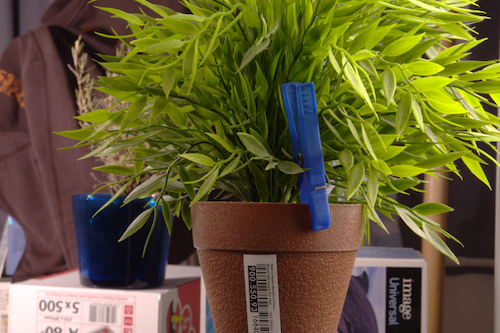
\includegraphics[width=\textwidth]{target.jpg}
        \caption{Plant Image}
    \end{minipage}
    \begin{minipage}{0.33\textwidth}
        
\includegraphics[width=\textwidth]{trimap.png}
        \caption{Plant Trimap}
    \end{minipage}
    \begin{minipage}{0.33\textwidth}
        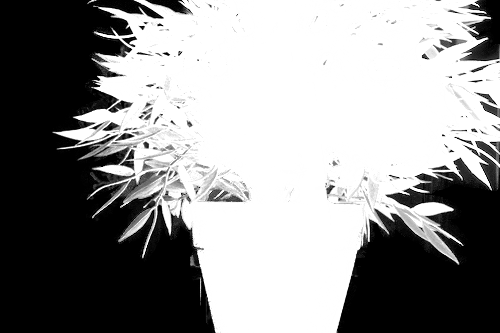
\includegraphics[width=\textwidth]{mask.png}
        \caption{Plant Soft Mask}
    \end{minipage}
\end{figure}

Once the alpha mattes are generated (soft mask) we can use them
to extract the object from the target image.
Thereore, we can remove the background behind the object,
fill the background with a color, replace it with another image
or leave it transparent.

Given a target image with pixels \(T_{x,y}\), the alpha
mattes \(\alpha_{x,y}\) and the pixels of the replacement image
\(R_{x,y}\) we can compute the pixels of the output image \(T_{x,y}'\)
as follows
\[
    T_{x,y}' = 
    \alpha_{x,y} \cdot T_{x,y} + (1 - \alpha_{x,y}) \cdot R_{x,y}
\]
If we want to replace the background with a color we can consider.
\(R={(r,g,b)}^t\) \\
If we just want to leave the background transparent, meaning
\(T' \in {\mathbb{R}}^4\), we have
\[
    T_{x,y}' = 
    \alpha_{x,y} \cdot T_{x,y}
\]
and the alpha value for \(T_{x,y}\) is set to \(\alpha_{x,y}\)

\pagebreak

\section{Opencv}

\begin{wrapfigure}{r}{3.5cm}
    
\includegraphics[width=3.5cm]{opencvlogo.png}
\end{wrapfigure}

OpenCV\cite{opencv} is a library
for computer vision. It contains a large
amount of tools, from GUIs, video analysis, machine learning,
object detection, image processing and many more\cite{opencvdoc}.
The library also contains a module about \textit{alpha matting},
contains a function to find generate alpha mattes given a trimap
\cite{opencvalphamatting}.

\wrapfill

Testo

\pagebreak

\listoffigures

\pagebreak

\nocite{*} % cite all entries

\printbibliography

\end{document}